% 信安大赛

% 小四 a4纸
\documentclass[12pt,a4paper]{ctexart}

% 插入常规居中图片
% 参数1:标准栏宽度的倍数 参数2:图片路径 参数3:图片脚注
\def\pic_normal#1#2#3{
\begin{figure}[H]
\centering
\includegraphics[width=#1\columnwidth]{#2}
\caption{\small{#3}}
\end{figure}
}

% 下划线加加粗
\newcommand{\important}[1]{\uline{\textbf{#1}}}

\usepackage{ctex}
% 设置列表数字类型
\usepackage{enumerate}
% 此包用于长表格换页
\usepackage{longtable}
% 此包用于设置缩进
\usepackage{indentfirst}
% 用于代码编辑
\usepackage{listings}
% 公式中可使用的便捷命令
\usepackage{amsmath}
% 中文下划线相关
\usepackage{CJKulem}
% 此包用于控制表格颜色
\usepackage[table]{xcolor}
% 定义代码中使用的颜色
\definecolor{commentgreen}{RGB}{2,112,10}
\definecolor{eminence}{RGB}{108,48,130}
\definecolor{weborange}{RGB}{255,165,0}
\definecolor{frenchplum}{RGB}{129,20,83}
% 此包用于添加更精细和丰富的下划线
\usepackage{ulem}
% 此包用于设置页边距
\usepackage{geometry}
% 此包用于设置插入图片
\usepackage{graphicx}
% 此包用于设置图片浮动
\usepackage{float}

\linespread{2}
\begin{document}

\lstset {
    language=C,
    frame=tb,
    tabsize=4,
    showstringspaces=false,
    numbers=left,
    breaklines=true,
    %upquote=true,
    commentstyle=\color{commentgreen},
    keywordstyle=\color{eminence},
    stringstyle=\color{red},
    basicstyle=\small\ttfamily, % basic font setting
    emph={int,char,double,float,unsigned,void,bool},
    emphstyle={\color{blue}},
    escapechar=\&,
    % keyword highlighting
    classoffset=1, % starting new class
    otherkeywords={>,<,.,;,-,!,=,~},
    morekeywords={>,<,.,;,-,!,=,~},
    keywordstyle=\color{weborange},
    classoffset=0,
}

%封面
\begin{titlepage}
 \newgeometry{left=3cm, top=8cm, right=3cm}
 \begin{center}
   \textbf{\zihao{1}2022年全国大学生信息安全竞赛作品报告}\\
 \end{center}
   \vspace{4cm}
   \textbf{作品名称:}
   \uline{“透镜”——基于Libbpf的鸿蒙OS平台隐私监测防护系统}\\
   \textbf{电子邮箱:} \uline{~~~~~~~~~~~~~~~gyz2019@whu.edu.cn~~~~~~~~~~~~~~~}\\
   \textbf{提交日期:} \uline{~~~~~~~~~~~~~~2022年6月5日~~~~~~~~~~~~~~~~~~~~~~~}


\end{titlepage}

% 恢复页边距
\restoregeometry

\tableofcontents
\newpage

\section{作品概述}
\subsection{背景分析}
从1983年GNU计划开始,过去四十年时间全球范围内仅仅有Unix和Linux两个真正建立起生态体系的操作系统。OpenHarmony承载使能千行百业的数字底座使命,站在巨人肩膀上奋力前行。\par
开源作为软件开发的基石,已经成为全球数字科技创新发展的大趋势。尤其是在基础软件行业,开源驱动了绝大多数技术的创新。世界进入万物互联,一款能跨终端、分布式的操作系统应运而生,华为在将名为“鸿蒙”的操作系统(HarmonyOS)开发出来之后,2020年、2021年分两次将基础能力代码捐献给开放原子开源基金会,以供开源之用,OpenHarmony项目由此诞生。\par
从2020年OpenHarmony开源项目成立以来,这款诞生于风雨之中,走向本土开源春天的操作系统就备受期待。围绕它有无数怀疑和冷眼,也有无数热血与希冀。两年过去,我们至少可以得出一个最基本的结论,OpenHarmony从来没有停下过前进的脚步。\par
如今,OpenHarmony正在构建面向消费电子、商用电子、工业电子市场终端设备生态,为包括个人消费、智慧城市、医疗、金融、能源、商业物联网、航空航天等行业提供统一融合的数字化创新基础平台,其能力覆盖家居、出行、运动健康、娱乐、办公、教育、社交购物、工业生产等等智能化场景。从我们熟悉的手机、家电、平板与PC、电视大屏、汽车,到市政照明、暖通、电梯等等行业终端,都可以成为OpenHarmony的舞台。\par
联接的需求无处不在,联接的障碍也随处可见。但OpenHarmony就是为此而生,走向开源仅仅是开始。OpenHarmony距离商业落地和生态繁荣、社区活力强劲,还需要完成一系列建设。
\begin{figure}[H]
\centering
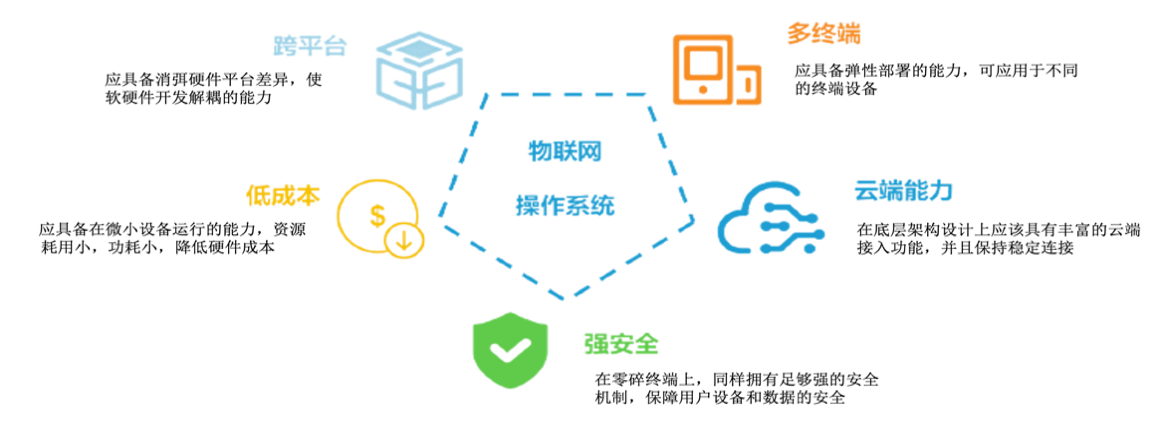
\includegraphics[width=0.8\columnwidth]{./pic/11.png}
\caption{\small{鸿蒙系统特性}}
\end{figure}
OpenHarmony实现万物互联的特有技术就是分布式软总线,分布式软总线技术将使终端设备打破硬件边界,让用户实现跨终端 无缝协同体验。以前硬件设备之间的连接及数据传输依靠的是硬总线,即物理导线。随着无线技术的发展,设备互联开始无线化。但是用户通常需要手动连接,存在连接时间长,连接及数据传输不稳定等问题。华为研发的分布式软总线技术在这一问题上进了改进,简化无线通讯协议,实现异构融合网络,使得无线连接性能无限逼近总线能力。在使用上,用户不再需要手动连接,设备之间能达 到自发现、自组网,端到端时延在 10 毫秒以内。连接建立之后,速度、延迟、稳定性都有改善,用户体验得到极大优化。在开发上,分布式软总线技术使得开发更为便捷,开发者开发多设备联动的应用时,无需关注组网方式与底层协议, 使开发者可以一次开发,多端部署。
\pic_normal{0.7}{./pic/12}{分布式软总线简化无线通讯协议}
两年多来快节奏的版本迭代,OpenHarmony系统能力、开发工具逐步完善,具备了满足大量产业需求的技术优势。虽然OpenHarmony距离真正的大规模商业落地还有一段路要走,但如今已踏出重要几步。OpenHarmony正在从聚光灯下出发,成为真正的基础软件,真正的开源操作系统。
\pic_normal{0.9}{./pic/13}{Openharmony支持设备演进历史}
penHarmony目前只具有基础的一些能力,但在隐私保护等方面还有所欠缺,且由于操作系统过新,目前相关领域工作较少。用户在上网过程中,身份信息泄露的途径有很多,最为常见的就是手机中的APP在后台擅自调用敏感权限来获取我们的个人信息。其中危害最大的莫过于软件偷偷打开摄像头对用户进行拍照或打开录音机对用户进行监听等。对此OpenHarmony还未在安全子系统中做任何的安全监控处理。


同时随着传统的内核跟踪工具的成熟,其各自自身的一些缺陷也渐渐成为了性能的瓶颈,同时部分跟踪工具还会影响内核的稳定性,这些问题亟需一项新技术来解决。也因此诞生了eBPF,eBPF的出现解决了上述两个主要问题,其监测效率高且不影响内核稳定性。但是由于不同内核版本之间的差别,会导致某个内核版本上编写的eBPF程序没法在另一个内核版本上完美运行。


基于以上背景和需求,本团队提出“透镜:基于libbpf的OpenHarmony隐私检测与防护系统”的作品方案,libbpf可以实现eBPF程序的CO-RE(Compile Once – Run Everywhere)。基于libbpf技术在内核层对摄像头、麦克风等设备进行监控,及时将后台的隐私行为数据进行分析和过滤,根据前端用户的需求将最终信息报告返回给用户。经过后期的系统测试,该产品还实现了轻量级、多内核版本、多平台可移植的特性目标。


\subsection{相关工作}
\subsubsection{eBPF相关技术}
\paragraph{eBPF概述}
eBPF 是一套通用执行引擎,提供了可基于系统或程序事件高效安全执行特定代码的通用能力,通用能力的使用者不再局限于内核开发者;eBPF 可由执行字节码指令、存储对象和 Helper 帮助函数组成,字节码指令在内核执行前必须通过 BPF 验证器 Verfier 的验证,同时在启用 BPF JIT 模式的内核中,会直接将字节码指令转成内核可执行的本地指令运行。


eBPF是一项革命性的技术,可以在Linux内核中运行沙盒程序,而无需更改内核源代码或加载内核模块。通过使Linux内核可编程,基础架构软件可以利用现有的层,从而使它们更加智能和功能丰富,而无需继续为系统增加额外的复杂性层。


eBPF导致了网络,安全性,应用程序配置/跟踪和性能故障排除等领域的新一代工具的开发,这些工具不再依赖现有的内核功能,而是在不影响执行效率或安全性的情况下主动重新编程运行时行为。

\paragraph{BCC技术}
BCC 是一个建立在 eBPF 基础上的高效内核跟踪和操作程序的工具包,它包括几个有用的命令行工具和例子。BCC 简化了用 C 语言编写 eBPF 程序的过程,包括一个围绕 LLVM 的封装器,以及 Python 和 Lua 的前端程序。它还提供了一个高层次的库,可以直接集成到应用程序中。


但是由于BCC 依赖于运行时编译,因此需要将整个庞大的 LLVM/Clang 库引入并嵌入到自身中。这会产生很多不理想的后果:编译期间占用大量资源,可能会中断繁忙服务器上的主要工作流程;依赖于内核头文件库,其必须安装在每个目标主机;即使是微不足道的编译时错误,也只能在重新启动用户空间程序之后的运行时才能检测到;显着增加了开发迭代时间。

\paragraph{BPFTrace技术}
bpftrace 是一个用于 Linux eBPF 的高级跟踪语言。bpftrace 使用 LLVM 作为后端,将脚本编译成 eBPF 字节码,并利用 BCC 作为与 Linux eBPF 子系统以及现有的 Linux 追踪能力和附件点进行交互的库。


但是由于bpftrace的语法过于简单,不能自定义函数,不能调用内核函数,所以只适合开发一些简单的小工具,并且无法实现内核级的系统监测。

\subsubsection{Hook技术}
\paragraph{内核态Hook}
~~~\newline
\textbf{SSDT Hook:}SSDT是系统服务描述符表,将Ring3的Win32 API和Ring0的内核API联系起来。SSDT不仅只包含一个庞大的地址索引表,还包含例如地址索引基地址、服务函数个数等其他重要信息。通过修改SSDT表的函数地址,可以对常用Windows函数以及API进行Hook,从而实现对目标系统动作进行过滤、筛选的目的,一些主机入侵防御系统、杀毒软件、系统监控、注册表监控软件往往会采用此接口来实现自身的监控模块。\\
\textbf{内核态的内联Hook:}Inline Hook首先通过特征码匹配验证内核API版本,通过硬编码的方式向内核API的内存空间写入跳转语句,接下来该API只要被调用,程序就会跳转到监控的函数中,监控函数需要完成3个任务:重新调整当前堆栈、执行遗失的指令、信息过滤。\\
\textbf{中断挂钩IDT Hook:}IDT(中断描述符表)用来处理中断,用户进程请求系统服务(SSDT)时,调用IDT中的0x2E,首先在系统中找到IDT,确定0x2E在IDT中的地址,并用构造的函数地址取代它,这样用户的进程——调用系统服务,设置的hook函数就会被触发。

\paragraph{用户态Hook}
~~~\newline
\textbf{IAT Hook:}PE文件中存在导入表,显示该模块调用的外部API。模块被加载进内存后,PE加载器会修改该表,将表中地址修改为外部API重定位后的真实地址,这时只需将地址修改为预置的新函数的地址,就可以完成对应API的Hook。\\
\textbf{Inline Hook:}Inline Hook通过修改API函数的代码,先将函数的前几个字节改为跳转指令,跳转到hook函数处,hook函数的最后一部分是原函数被修改的指令跳转到原函数的指令,以此来实现对API的监控。


IAT Hook技术技术虽然能够挂钩几乎所有静态调用的API函数,但也会存在缺陷,动态调用的API函数在进行跳转时不经过IAT,也就无法对此类调用进行拦截。例如当通过LoadLibrary和GetProcAddress来加载DLL调用API时,IAT Hook将不会产生作用,导致监控函数调用的失败,进而降低进程注入攻击的检测率。\\
\textbf{ptrace API调试技术Hook:}ptrace是很多Linux平台下调试器实现的基础,包括syscall跟踪程序strace。


使用ptrace的总体思路为
\begin{enumerate}
  \item ptrace attach目标进程。
        \item 保存rip
        \item 控制跳转到mmap分配一段rwx内存
        \item 将一段机器码copy进去
        \item 控制跳转到机器码(可以以bin文件的形式)
        \item 恢复执行。
\end{enumerate}


这种方式实现的跟踪工具有很多的限制,同时性能也不够优秀。


因此,总体来讲,现有方法在检测进程注入攻击方面存在检测率低、检测点滞后等问题。

\subsection{竞品分析}
目前国内基本没有在OpenHarmony上的用户隐私保护工作,故我们分析了一些其他平台上的隐私保护软件。


\vspace{0.3cm}
\begin{table}
\begin{tabular}{|p{3cm}|p{6cm}|p{3cm}|}
  \hline
  \rowcolor{blue!50} 应用名称&服务内容&特点分析\\
  \hline
  火绒安全-摄像头保护(Windows)&发现并提示应用程序开启摄像头&电脑软件,检测目标单一,重复开启不提示\\
  \hline
  镜头盖APP(Android)&手动禁用摄像头&控制对象单一,只能直接禁用而付费监测\\
  \hline
  摄像头和麦克风拦截者(Android)&\begin{enumerate}
                                  \item 手动禁用摄像头和麦克风
                                  \item 根据日期/位置禁用摄像头和麦克风
                                        \item 白名单
                                \end{enumerate}&只能直接禁用,而非监测\\
  \hline
\end{tabular}
\caption{其他平台上的隐私保护软件}
\end{table}

从上表可知,目前移动端的摄像头等隐私行为保护大多使用手动禁用的方式来保护,但这样的方式不够灵活,且是在应用层的防护。我们想要实现一个可以在多内核版本、多类型平台都可以进行内核级隐私检测行为的轻量级应用。

\subsection{特色描述}
首先系统特性方面,我们的作品是建立于鸿蒙OS——OpenHarmony上的,该系统为国产自研Linux内核系统,近几年才兴起火热。其系统新,故而也存在很多问题,比如资料匮乏、文件不完善、接口少、框架应用不足等。尤其是位于底层的隐私监测系统,此前未有研究人员在此方向尝试;而且尽管其它系统平台有不少成熟的应用,但都不能简单地移植过来,不具备兼容性与可行性。也正因如此,我们的作品应运而生。


其次内核交互方式上,我们所采用的是基于Libbpf的应用框架,libbpf相较于传统的BCC有着非常突出的优势,包括内存占用少、编译更加方便快速等等。我们通过它,可以在内核中监测到大量的系统调用行为,并通过一系列数据处理最后获得我们想要监测的使用情况、隐私数据,上传给前端。


而我们的框架与属性优势主要体现在两点上,第一点我们的系统应用检测框架具有\uline{\textbf{可拓展性}},其不仅仅局限于我们当前实现了的隐私行为监测,之后还可以进行拓展扩充,通过在已有框架中添加模块的方式,监测其它诸如应用安装、后台权限等等更多的应用程序行为,从而实现更全面的安全性覆盖。第二点是我们的系统架构具有\uline{\textbf{可移植性}},这也是Libbpf的CO-RE理念核心所在,其编译一次便可以运行于许多版本的内核中,经过我们的测试,只需要简单修改上层接口,便可以很好地运行于其它系统,比如Linux与Android。

\subsection{前景分析}
随着网络技术的不断发展,互联网安全对国家、社会及个人的重要作用日益彰显。针对当前互联网安全面临着的巨大压力,新技术的应用与研究是解决这类问题的关键。


与此同时,鸿蒙系统的出现于快速发展代表着我国互联网技术的一次巨大飞跃,但鸿蒙系统的开发仍有不足之处,系统安全性和完整性仍需不断完善。本次项目实现的“透镜”工具实现了在Linux内核下对用户隐私行为的实时监测,并将其移植到鸿蒙系统中进行应用,提高了移动设备系统的安全性,在个人隐私受到各方面威胁的当下具有深远意义。


同时该系统检测工具具有移植性,可以移入到不同的内核版本与移动设备中,并且除了设备检测外还可以加入检测用户数据和网络流量等其他模块。这代表着该应用仍有很大的完善空间,可以实现更加全面、详细、个性化的系统检测服务。
\pic_normal{0.8}{./pic/14}{鸿蒙未来发展前景(1)}
\pic_normal{0.8}{./pic/15}{鸿蒙未来发展前景(2)}

\subsection{专业术语}
\newpage
  \begin{longtable}{|l|p{10cm}|}
    \hline
    名称&概念\\
    \hline
    kprobe机制&kprobe是Linux内核的一个重要特性,是一个轻量级的内核调试工具。其不需要重新编译内核代码,因而相比于原始的printk代价更小、效率更高。同时它还是其他一些更高级的内核调试工具的基础,之后兴盛的eBPF也同样依赖于kprobe。kprobe可以让用户在内核几乎所有的地址空间或函数(某些函数是被能被探测的)中插入探测点,用户可以在这些探测点上通过定义自定义函数来调试内核代码。\\
    \hline
tracepoint追踪点 & tracepoint是内核预先定义的静态探测点,分布于内核各子系统中,可以用于挂载钩子函数实现trace功能。当没有钩子函数时,它几乎没有损耗,只有挂载了钩子函数才会真正启用trace功能。这个被挂载的钩子函数由开发者编写内核module实现,并且在其中我们获取调试所需要的信息并导出到用户态,这样就可以根据需要获取内核运行时的信息。 \\
\hline
ACE              & ACE(Ability Cross-platform Environment)开发框架,作为ACE框架的轻量实现,提供了一套跨平台的类web应用开发框架,通过Toolkit将开发者编写的HML、CSS和JS 文件编译打包成JS Bundle,然后再将JS Bundle解析运行成C++ UIKit的View 组件进行渲染。 \\
\hline
Napi             & Node-Api是用于封装JavaScript能力为native插件的API,独立于底层JavaScript,并作为Node.js的一部分。 支持的能力 Node-API可以去除底层的JavaScript引擎的差异,提供一套稳定的接口。 \\
\hline
KAL              & 鸿蒙的内核抽象层(KAL,Kernel Abstract Layer)通过屏蔽多内核差异,对上层提供基础的内核能力,包括进程/线程管理、内存管理、文件系统、网络管理和外设管理等。 \\
\hline
HAP              & HarmonyOS应用发布形态为APP Pack(Application Package,简称APP),它是由一个或多个HAP(HarmonyOS Ability Package)包以及描述APP Pack属性的pack.info文件组成。HAP是Ability的部署包,HarmonyOS应用代码围绕Ability组件展开,它是由一个或多个Ability组成。Ability分为两种类型:FA(Feature Ability)和PA(Particle Ability)。FA/PA是应用的基本组成单元,能够实现特定的业务功能。FA有UI界面,而PA无UI界面。 \\
\hline

  \end{longtable}


\section{作品设计与实现}
\subsection{系统架构}
\subsubsection{系统整体结构图}
系统整体架构图如下所示:
\pic_normal{1}{./pic/21}{系统整体结构图}

我们的系统主要按照三层逻辑结构进行组织,从上到下依次为应用层、框架层以及底部的内核层。而我们的工作主要分为前端与后端两块,并分别立足于应用层和框架层,并实现与内核层的交互。


在应用层部分,我们主要基于鸿蒙OS——OpenHarmony,利用建立于JS引擎上的ACE UI框架,编写GUI界面,构建我们的前端应用程序。


而在框架层部分,我们实现了一个完整的以NAPI为主要工具和接口的系统检测框架,该框架具有可拓展性与可移植性,不仅适用于我们的鸿蒙OS系统,同时也可以运行于Linux与Android系统,在其上我们可以添加各种功能丰富的模块。


并且我们还以Libbpf为核心编制了一个能够检测应用程序对隐私内容访问情况的隐私监测模块,该模块运行于框架层,并可以藉由Libbpf与内核互动,从中轻量级地获取系统调用数据,并对这些数据进行处理后返回给前端。该模块可以监测的对象包括系统设备(摄像头、麦克风、音响、GPS定位等)、网络数据(流量情况、浏览行为等)以及用户数据(个人信息、系统本地文件等),功能十分的强大。


最底部的内核层主要为上层服务,其基于Linux内核与鸿蒙的LiteOS架构,以实现KAL内核级抽象,为我们工作的框架层与应用层提供数据。

\subsubsection{系统实现难点}
\paragraph{兼容性}
本产品最初的底层隐私检测代码实现、以及后续的开发测试环境均为Linux系统,而我们最终想要实现的是OpenHarmony系统环境下的移动应用。尽管OpenHarmony是基于Linux内核,但是其中的很多头文件和模块都已经被删除或者修改,这对我们系统移植的过程提高了难度。


同时,在OpenHarmony系统中实现前后端接口调用与数据交互时,也与Linux环境或Andriod环境下有很大不同。针对不同的系统我们需要在不同的接口层上进行函数接口暴露以及函数间数据互通。本产品中我们实现了基于NAPI的鸿蒙系统检测应用框架,通过NAPI接口实现前后端的相互调用。

\paragraph{可用性和安全性之间的平衡}
由于本作品是一个系统级监测隐私行为的软件,在监测隐私行为和保护用户行为时,如何兼顾应用原本的可用性是一个重要问题。在这里,我们将可用性分为两个方面:一个是本作品的用户体验,另一个是被监测应用的原本功能是能正常执行。


本作品通过在内核层面监控有关摄像头、麦克风等设备的打开、关闭等行为来判断是否发生隐私行为。以摄像头为例,正常的相机软件和非正常的隐私窃取行为,一旦调用了摄像头就会触发我们在内核插桩点中插入的函数,从而我们能得知隐私行为正在发生。虽然这样的方法能监测所有隐私行为,但是无法区分正常的调用和非正常的恶意隐私窃取。如果每一次调用都反馈给用户,则会导致系统弹窗过多,给用户的体验感不佳,因此还需要用其它方法来甄别合法行为和不合法行为,并只报告不合法行为,这是我们需要解决的难点之一。


其次,在用户获知不合法的隐私行为后,如何解决禁止不合法的隐私行为且不影响该应用原本的功能。据我们所知,一些应用在使用之初会获取用户对某些行为的授权,若用户不允许则可能导致该程序无法正常使用。因此,禁止隐私行为的发生同时保证被监测应用的可用性也是我们需要解决的一个难点。

\subsection{关键技术}
\subsubsection{基于NAPI的鸿蒙系统检测应用框架}
\paragraph{介绍}
这部分我们实现的是一个实现系统检测功能的\important{整体应用框架}。该框架以NAPI为主要的系统接口,从而能够在OpenHarmony系统上运行。之后我们还会通过添加\important{可移植性的方案}使其能够运行于其它操作系统,比如Android。

\paragraph{应用流程}
首先,用户在进程空间通过访问我们的前端应用程序,在ACE UI界面中选择其想要进行监控的服务或者输入某种指令,这些行为与数据将通过NAPI的接口开启我们的隐私检测服务,并最终传入到后台。而我们的程序开启后会始终于后台运行。


我们的应用程序会在其运行中分析系统的设备情况,通过分析行为,获取不同设备在被使用过程中打开文件、关闭文件、退出进程的\important{系统调用函数},并且在这些函数的前后进行\important{插桩}。这样当其它应用程序访问或者使用该系统设备时,就会进行系统调用从而通过插桩点进入到与内核交互的\important{Libbpf流程}当中,获取数据。


数据最后传回到数据处理模块,并将最终的结果呈现给用户。
\pic_normal{0.9}{./pic/22}{应用框架图}

\paragraph{NAPI}
Napi用于L2设备支持的JS API实现。Napi在系统中的位置位于框架层的顶层。
\pic_normal{0.9}{./pic/23}{NAPI结构图}

\begin{enumerate}
  \item 模块注册

        API集合按业务功能进行模块划分。开发者使用前须import对应的模块。
命名方式为@ohos.模块名。
注册过程中需要注意的是:模块名须唯一,由ACE团队统一维护,子系统新增模块时须向ACE团队申请。模块名最好是单个名词。实在不行,也可以由多个名词组成,但必须遵循小驼峰命名规则。一个模块,一个声明文件(*.d.ts)。声明文件命名遵循@ohos.模块名.d.ts,文件名全小写,单词间无分割。
NAPI通过注册函数进行模块的注册,其接受一个全局变量参数,全局变量结构体中定义了模块名及模块初始化函数。在模块的初始化中,我们可以定义模块需要暴露的方法及属性。

  \item NAPI实现
        \pic_normal{0.8}{./pic/24}{NAPI调用流程图}

        其实现方式有两种,一种通过c一种通过c++。


        区别如下图所示:
        \pic_normal{0.8}{./pic/25}{NAPI的不同接口区别}
        NAPI有关的接口信息可以在Node.js官方文档中查看,在这里我们主要使用C接口在实现过程中主要使用的接口如下

\end{enumerate}

\subsubsection{基于Libbpf的hook模型}
\paragraph{eBPF的工作原理}
eBPF 程序在事件触发时由内核运行,所以可以被看作是一种函数挂钩或事件驱动的编程形式。事件可由 kprobes/uprobes、tracepoints、dtrace probes、socket 等产生。这里选用tracepoints,主要原因在于。这允许在内核和用户进程的指令中钩住(hook)和检查任何函数的内存、拦截文件操作、检查特定的网络数据包等等。


事件触发了附加的 eBPF 程序的执行,后续可以将信息保存至 map 和环形缓冲区(ringbuffer)或调用一些特定 API 定义的内核函数的子集。一个 eBPF 程序可以链接到多个事件,不同的 eBPF 程序也可以访问相同的 map 以共享数据。一个被称为 “program array” 的特殊读/写 map 存储了对通过 bpf() 系统调用加载的其他 eBPF 程序的引用,在该 map 中成功的查找则会触发一个跳转,而且并不返回到原来的 eBPF 程序。这种 eBPF 嵌套也有限制,以避免无限的递归循环。


运行 eBPF 程序的步骤:
\begin{enumerate}
  \item 用户空间将字节码和程序类型一起发送到内核,程序类型决定了可以访问的内核区域(主要是 BPF 辅助函数的各种子集)。
  \item 内核在字节码上运行验证器,以确保程序可以安全运行(kernel/bpf/verifier.c)。
  \item 内核将字节码编译为本地代码,并将其插入(或附加到)指定的代码位置。(如果启用了 JIT 功能,字节码编译为本地代码)。
  \item 插入的代码将数据写入环形缓冲区或通用键值 map。
  \item 用户空间从共享 map 或环形缓冲区中读取结果值。
\end{enumerate}\par
map 和环形缓冲区结构是由内核管理的(就像管道和 FIFO 一样),独立于挂载的 eBPF 或访问它们的用户程序。对 map 和环形缓冲区结构的访问是异步的,通过文件描述符和引用计数实现,可确保只要有至少一个程序还在访问,结构就能够存在。加载的 JIT 后代码通常在加载其的用户进程终止时被删除,尽管在某些情况下,它仍然可以在加载进程的生命期之后继续存在。


为了方便编写 eBPF 程序和避免进行原始的 bpf()系统调用,内核提供了方便的 libbpf 库,包含系统调用函数包装器,如bpf\_load\_program(用于将BPF程序挂载到内核中) 和结构定义(如 bpf\_map)

\paragraph{基于eBPF的监测框架}
目前eBPF的各种监测工具很多,但是对于不怎么接触eBPF的开发者来说,还没有一个比较容易使用的监测设备使用的接口。我们构建了一个对于设备的监测框架,利用eBPF在底层hook对设备文件的读写操作。在hook设备文件的跟踪程序类型上我们选择比较稳定的tracepoints作为我们eBPF程序的程序类型。tracepoints 是内核开发人员维护的跟踪点,能够提供稳定的 ABI 接口,一般不会因为内核版本的变化而导致跟踪失效。获取到内核中的数据后,对数据进行过滤,去重,筛选,最终给出使用设备的进程相关数据。向外暴露获取设备使用数据的接口,开发人员只需要通过接口读取数据即可按照自己的意愿进行处理。这样屏蔽了eBPF的底层实现,在充分利用eBPF的高效率的基础上提供了极大的可扩展性,大大降低了基于eBPF开发监测设备使用等相关测试工具的开发难度。

\subsubsection{基于F3N的行为检测分析弹性机制}
\paragraph{概述}
在监测应用使用设备的过程中。若每当有应用使用设备时就给出用户提示,当用户正常使用设备时,如打开照相机进行拍照,这种提示会影响用户的体验。因此需要对应用使用设备行为进行分析。可以通过构建一个应用行为模型,将应用恶意或正常使用设备的行为特征作为训练数据。同时在用户许可的情况下让用户判断应用在哪些情况下使用设备的行为是恶意的,并将这部分数据共享给服务端,之后服务端可使用这些数据做进一步的分析,从而不断完善模型,实现自适应的性能提升。
\pic_normal{0.6}{./pic/26}{系统客户端与服务端的交互}

\paragraph{模型阐述}
在鸿蒙系统上,我们构建一个分布式跟踪和执行模块作为守护程序集。策略会跟随应用程序的生命周期,而不是永久地运行在基础设施上。这点与sidecar相似,但我们基于高性能的Libbpf实现,不需要将能力重定向到sidecar中,从而降低系统开销。


基于此,我们实现了在鸿蒙系统上的结合智能策略、集中管理、自动发现于一体的完整监测防护系统,能够对用户行为进行自动的分析,并使用弹性补丁,来及时限制应用的权限和能力,以防止恶意攻击行为。这类似于在应用程序周围放置一个防护罩,将漏洞限制在本地防护罩内,并且不允许传播。


凭借与服务器定时的连接与更新,在本地运行的所有策略都可以实现自动发现与自我纠正。针对于应用越级行为的解决方案,具备自动化特性,可以消除用户人为操作错误等因素,这将大大提高了我们作品应用的便捷性、准确性、安全性。通过人工智能的相关方式,利用多用户网络构建的应用分析数据,建立行为模型,持续监控系统设备、网络行为,并在持续运行的过程中不断学习,提升模型准确性,最后搭建完成一种能够自适应变化提升的弹性防护机制。

\pic_normal{0.8}{./pic/27}{对应用的权限限制}
为了提高应用行为分析的效率,我们会在本地保存模型数据,该模型版本从云端下载,保持定时的更新,而更新的频率可以为用户自定义设置。同时本地实时的处理过的数据,在用户授权允许的情况下,也会定时地传送给服务器,以供模型的训练与自适应提升。


交互图

行为数据特征

过利弊权衡,我们选择的分析数据包括:应用获取数据的流向、发送的网络包特征、调用设备频率、后台占用率等,通过归一化的方式构建向量,采用无监督的聚类学习来进行模型训练。


之所以没有先采用有监督学习模型的原因是数据的标注难度比较大,且当前该领域没有合适的、成型的数据集。在后续的工作中,我们会尝试自己采集数据、标注数据来训练精度更高的模型。

神经网络的选取:


选择的是FNN模型,它在提出之时是用于进行用户的点击行为预测的,这里我们通过调整,使其可以实现预测应用行为恶意倾向的作用,我们称之为F3N(FNN NEW)。

在广告预测中,定位技术都依赖于预测是否特定的用户认为这个广告是相关的,给出用户在特定的场景中点击的概率,而我们的F3N可以计算出应用程序在一个场景中行为恶意的倾向性,也就是其被预测为恶意的期望值。


目前大部分预测的线性模型,如逻辑回归,朴素贝叶斯,FTRL逻辑回归和贝叶斯逻辑回归等,都是基于使用one-hot编码的大量稀疏特征,模型简单有效,但是由于无法学习到特征之间的相互关系,性能较差。而非线性模型可与其相比,可以通过特征间的组合提高模型的能力,比如FMs将二值化的特征映射成连续的低维空间,通过内积获取特征间的相互关系。然而,这些方法并不能利用所有可能的组合。此外,许多模型仍然需要依靠手工进行特征工程,来决定如何进行特征的组合。另一个问题是,一些已有的模型在对复杂数据间的潜在的模式上的表达能力是非常有限的,这也影响到它们的泛化能力。这也是为什么我们选择了FNN作为我们模型的前身,经过改进和适配形成新的模型F3N。


在非监督的训练中,神经网络可以从原始的特征中学习到高维的特征表示,这个能力也可以用在应用行为分析上。我们模型的输入特征如前所述,是不同领域的并且离散的类别特征,包括后台占用率、网路数据包、数据流向等等,并且特征之间的相互依赖是未知的,这也对我们的模型提出了挑战。
\pic_normal{1}{./pic/28}{FNN模型结构图}
输出层,模型的输出是一个实数y(0,1)作为预测的概率,即应用在指定上下文中行为是恶意的概率。
\begin{equation}
\hat{y}=\operatorname{sigmoid}\left(\boldsymbol{W}_{3} \boldsymbol{l}_{2}+b_{3}\right)
\end{equation}
l2层
\begin{equation}
\boldsymbol{l}_{2}=\tanh \left(\boldsymbol{W}_{2} \boldsymbol{l}_{1}+\boldsymbol{b}_{2}\right)
\end{equation}
l1层
\begin{equation}
\boldsymbol{l}_{1}=\tanh \left(\boldsymbol{W}_{1} \boldsymbol{z}+\boldsymbol{b}_{1}\right)
\end{equation}
Dense层
\begin{equation}
\boldsymbol{z}_{i}=\boldsymbol{W}_{0}^{i} \cdot \boldsymbol{x}\left[\operatorname{start}_{i}: \operatorname{end}_{i}\right]=\left(w_{i}, v_{i}^{1}, v_{i}^{2}, \ldots, v_{i}^{K}\right)
\end{equation}

其中start和end是第个特征域的起止下标,w和x在上面已经描述过了。所有的权重w都是通过偏置项wi和向量vi分别初始化。通过这种方式,FNN中的第一层的参数向量z就是通过预训练好的FM模型来初始化的。

\subsection{系统实现}
\subsubsection{基于libbpf的内核级隐私检测Hook模块}
\paragraph{介绍}
这一部分是我们底层应用架构的核心,涉及系统中框架层与内核层的交互。实现主要依托于Libbpf,分为.c和.bpf.c两个文件,分别用于\important{启动检测}、与内核进行交互\important{获取内核中得到的数据},以及对得到的数据进行\important{过滤、去重、统计、分类、函数封装}等处理。最后这些处理好的数据与函数还会再向上传递,以供上层NAPI以及前端的使用。
\pic_normal{0.8}{./pic/29}{hook模块结构图}

\newgeometry{bottom=0.5cm}
系统内核与设备的交互是依赖于\important{设备驱动程序}的,而系统中绝大部分设备的驱动程序都在\important{device目录}下,所以我们可以利用这一点,通过监测程序访问驱动文件的行为,来监测其对设备的使用。


可监控设备的设备有:摄像头、麦克风、声卡、GPS定位等等,也可以通过修改底层代码以添加更多的监测对象。


本质来说我们撰写的是一个模块,其对应的功能是监测鸿蒙OS中应用进程对设备的使用情况,当然之后也可以对功能进行拓展,撰写其它的模块实现更多更强大的功能,这些模块都可以被很方便地置于我们所自主构建的应用框架当中。所以模块的\important{可拓展性与可移植性}是本项目的突出特色之一。

\paragraph{数据处理}
这部分首先要设置strict模式,之后加载并检验BPF程序,添加tracepoint插桩点,设置ring缓冲区.


之后将我们的程序handle附着到hook锚点上,从而使得BPF程序能够相应,在其拥有的上下文context中回应系统调用、执行我们的代码,从而获取与设备驱动程序文件相关的内核数据。


这些数据会被储存在缓冲区当中,之后我们调用数据处理模块,最后清空缓冲区。


数据处理模块流程图:
\pic_normal{0.8}{./pic/210}{数据处理模块流程图}
下面是对各数据处理部分的具体介绍:

\begin{enumerate}
  \item 过滤

过滤主要是为了获得与系统驱动目录下的文件有关的系统调用服务。


过滤方式依靠字符串处理函数,比较进程行为中打开或者关闭的文件名与已知关键词之间的相关性,来得到进程名称,之后还可以对不涉及文件名的进程行为,比较其进程名称与已知的涉及设备访问的进程名称的相关性。

部分文件名与设备对应表格:


\begin{table}[htb]
\centering
\begin{tabular}{|p{4cm}|p{2cm}|p{3cm}|}
  \hline
  \rowcolor{blue!50} 文件名&操作&设备\\
  \hline
   /dev/video*&读/写&摄像头\\
  \hline
  /dev/snd/pcmC0D0&读&麦克风\\
  \hline
  /dev/snd/pcmC0D0&写&音响\\
  \hline
  /dev/snd/pcmC0D1&写&音响\\
  \hline
  /dev/snd/pcmC1D0&读&麦克风\\
  \hline
  /dev/snd/pcmC1D0&写&音响\\
  \hline
  /dev/snd/pcmC1D1&写&音响\\
  \hline
  /dev/snd/pcmC2D0&读&麦克风\\
  \hline
  /dev/snd/pcmC2D1&写&音响\\
  \hline
\end{tabular}
\caption{其他平台上的隐私保护软件}
\end{table}
\restoregeometry
  \item 去重


去重是在过滤之后(从运行逻辑上来说也可以放在过滤之前),因为libbpf监测的灵敏性,短时间内可以获得到大量的系统内核级行为以及数据,同时也就意味着大量的重复,所以需要进行去重处理。


我们的去重标准比较简单,基本就是两点,第一点是连续的完全相同的行为记录,只保留一条;第二点是在第一点去重之后,行为分析结果相同的两条,如果时间相隔太近,也依然只保存一条,这是因为从用户需求的角度来说,用户是不需要短时间内重复的提示的。

  \item 统计与分类

统计与分类几乎是同时进行的。统计是针对于过滤去重后的数据,进行相应的数学统计,比如统计当前有多少个进程在使用声卡进行音频的播放,有多少应用程序试图或者正在使用摄像头。


而分类主要是对检测到的行为类别进行划分,比如该调用行为是针对于哪一个设备,其是否正常合法、是否占用时间过长等等。

  \item 封装

封装是为了方便于上层界面,使得上层可以直接根据其具体的需要调用相应的函数。

\end{enumerate}


\paragraph{启动检测}

这部分主要是通过libbpf库中的一些函数实现与底层内核态之间的交互。


bpf程序与内核交互过程:

\pic_normal{0.8}{./pic/211}{bpf程序与内核交互图}

首先我们更新Maps结构,创建ring buffer缓冲区,并从缓冲区中保存空样本。


之后当通过verifier检验后,在内核中我们插桩好的BPF静态追踪点tracepoint上,我们运行挂载的程序(比如处理打开文件的handld\_exec),从而获取锚点上下文ctx,然后利用libbpf封装好的库函数,我们可以获取到我们想要的数据,包括时间戳、进程名、文件名等。


比如通过bpf\_get\_current\_pid\_tgid()我们可以获得当前进程名称,通过bpf\_ktime\_get\_ns()可以获取系统时间戳。


之后需要往之前的空样本中填充数据,分别利用bpf\_get\_current\_comm()从上下文中获取进程名并填充,利用bpf\_probe\_read\_str()从上下文中获取文件名并填充。


最后我们通过bpf\_ringbuf\_submit()提交缓冲区将数据传递给数据处理部分(用户态)。


监控打开文件的程序流程图:

\pic_normal{0.8}{./pic/212}{监控打开文件程序流程图}

之后对于关闭文件与进程退出,分别执行大致相同的操作。主要的区别在于插桩的内核BPF锚点不同,以及由于上下文不同,其所能够获取到的数据的内容有些微不同,这些可以根据需要进行调整。


详细的代码内容可以在后续\important{《具体实现》}中查看。

\subsubsection{隐私监测模块部分代码}
\paragraph{bpf部分代码}
这里所呈现的是我们系统实现后端中的部分代码,test.bpf.c是一个以.bpf.c为后缀的C语言文件,其前面的名称不重要。这部分代码实现的是对于系统监测服务的启动、从内核中获取数据,并传递给用户空间的功能,对应于前面介绍到的“启动监测”部分。

引入头文件:

\begin{lstlisting}
#include "final_test.h"
#include "vmlinux.h"
#include <bpf/bpf_core_read.h>
#include <bpf/bpf_helpers.h>
#include <bpf/bpf_tracing.h>
\end{lstlisting}

证书声明:
\begin{lstlisting}
char LICENSE[] SEC("license") = "Dual BSD/GPL";
\end{lstlisting}
LICENSE变量定义了BPF代码的许可证。指定许可证是强制性的,由内核强制执行。某些 BPF 功能不可用于非 GPL 兼容代码。


Maps结构的定义:
\begin{lstlisting}
struct {
  __uint(type, BPF_MAP_TYPE_HASH);
  __uint(max_entries, 8192);
  __type(key, pid_t);
  __type(value, u64);
} exec_start SEC(".maps");

struct {
  __uint(type, BPF_MAP_TYPE_RINGBUF);
  __uint(max_entries, 256 * 1024);
} rb SEC(".maps");
\end{lstlisting}

Map实际上是一个global全局变量,这也就是BPF的主要功能体现所在。 它定义了这样一个global变量SEC,BPF代码可以读取和更新,就像任何用户空间C代码一样。使用 BPF global变量来维护 BPF 计划的状态非常方便,而且性能也非常出色。此外,此类global变量可以从用户空间方面读取和编写。


下面重点介绍打开文件时的函数handle\_exec的执行原理与流程。该函数将被加载到内核的bpf程序中。


而在函数定义之前,需要设置插桩位置。该插桩位置(tracepoint)为进入系统调用openat时。这也是我们区分监测不同系统调用函数时具体处理功能差异的主要依据。
\begin{lstlisting}
SEC("tp/syscalls/sys_enter_openat")
\end{lstlisting}

这里的参数选择时进入系统调用时的上下文ctx。
\begin{lstlisting}
int handle_exec(struct trace_event_raw_sys_enter *ctx)
\end{lstlisting}

首先定义各种需要的结构和变量,包括task、事件e,进程号和u64时间。
\begin{lstlisting}
  struct task_struct *task;
  int fname_off;
  struct event *e;
  pid_t pid;
  u64 ts;
\end{lstlisting}
调用bpf\_get\_current\_pid\_tgid函数来获取进程号。


调用bpf\_ktime\_get\_ns函数获取当前时间。


此部分将PID(或内部内核术语中的"TGID")编码为32位的返回值。然后,它会检查触发syscall的进程是否是我们的进程,这在繁忙的系统中非常重要,因为可能会检测到很多不相关的进程。全球变量my\_pid将由用户空间那边的代码传输进来。
\begin{lstlisting}
  pid = bpf_get_current_pid_tgid() >> 32;
  ts = bpf_ktime_get_ns();
  bpf_map_update_elem(&exec\_start, &pid, &ts, BPF\_ANY);
\end{lstlisting}
设置最小时间单元,单位为纳秒。
\begin{lstlisting}
  if (min_duration_ns)
    return 0;
\end{lstlisting}
从缓冲区中获取样本保存为变量e,如果获取失败,退出程序。
\begin{lstlisting}
  e = bpf_ringbuf_reserve(&rb, sizeof(*e), 0);\\
  \setlength\parindent{1em}
  \indent
  if (!e)\\
  \setlength\parindent{4em}
  \indent
    return 0;
\end{lstlisting}
获取当前的任务task,向样本中填充数据。
\begin{lstlisting}
  task = (struct task_struct *)bpf_get_current_task();
\end{lstlisting}

分别填充定义的样本e的各部分内容,设置exit\_event的值,用于区分文件的打开与关闭行为,0表示非退出,1表示退出;设置pid值为之前获取到的进程号;设置ppid为填充的task的tgid值;设置文件描述符fd为上下文中的参数列表首项;
\begin{lstlisting}
  e->exit_event = 0;
  e->pid = pid;
  e->ppid = BPF_CORE_READ(task, real_parent, tgid);
  e->fd = ctx->args[0];
\end{lstlisting}

获取进程名称与文件名称。
\begin{lstlisting}
  bpf_get_current_comm(&e->comm, sizeof(e->comm));\\
  \setlength\parindent{1em}
  \indent
  bpf\_probe\_read\_str(&e->filename, sizeof(e->filename),
  (void *)ctx->args[1]);
\end{lstlisting}
将已经填充好了数据,整个过程顺利执行的缓冲区提交给用户空间,以供后续的数据处理。
\begin{lstlisting}
  bpf_ringbuf_submit(e, 0);
\end{lstlisting}


\paragraph{用户空间部分}
这里所呈现的则是我们系统实现后端中的另外一部分代码,test.c是一个标准的以.c为后缀的C语言文件,与正常程序没有太大差别,也可以使用通常的各种系统C语言库。同样,其前面的名称test并不重要。


主要包括链表节点的创建、插入、修改、删除,针对于字符串的数据处理,包括过滤、去重、分类、统计等,以及对各函数的整体封装。


同时针对于不同类型的系统设备,定义有不同的处理函数。如果想根据具体的系统特性添加设备,只需要复制一份处设备处理函数然后更改设备名即可。


以视频处理函数为例,该函数名为video\_conduct:
\begin{lstlisting}
//视频处理
void video_conduct(const struct event *e) {
  // struct record_event record_new;
  int dev_type = 1; // video
  struct record_event *ptr = record_search(e->pid, dev_type, head);
  if (e->exit_event == 0) {
    if (ptr == NULL) {
      struct record_event *record_new = record(1, e);
      if (eno == 0) {
        head = record_init(record_new);
      } else {
        record_insert(head, record_new);
      }
      eno++;
      //系统提示
      modal(record_new, 1, dev_type);
    } else {
      ptr->fd[e->fd] = 1;
      ptr->stack++;
    }
  } else {
    if (ptr == NULL) {
      printf("error, process not exit!\n");
      return;
    } else {
      use_over(ptr, 0);
    }
  }
}
\end{lstlisting}

\subsubsection{基于方舟开发框架的前端设计}
\paragraph{方舟开发框架概述(ArkUI)}
方舟开发框架,是一套UI开发框架,提供开发者进行应用UI开发时所必须的能力,框架结构如下图所示。从图中可以看出,方舟UI开发框架支持两种前端开发范式:类Web开发范式与声明式开发范式。
\begin{itemize}
  \item 类Web开发范式

类Web开发范式,采用经典的HML、CSS、JavaScript三段式开发方式。使用HML标签文件进行布局搭建,使用CSS文件进行样式描述,使用JavaScript文件进行逻辑处理。UI组件与数据之间通过单向数据绑定的方式建立关联,当数据发生变化时,UI界面自动触发更新。此种开发方式,更接近Web前端开发者的使用习惯,快速将已有的Web应用改造成方舟开发框架应用。主要适用于界面较为简单的中小型应用开发。
        \item 声明式开发范式

声明式开发范式,采用TS语言并进行声明式UI语法扩展,从组件、动效和状态管理三个维度提供了UI绘制能力。UI开发更接近自然语义的编程方式,让开发者直观地描述UI界面,不必关心框架如何实现UI绘制和渲染,实现极简高效开发。同时,选用有类型标注的TS语言,引入编译期的类型校验,更适用大型的应用开发。本作品使用了声明式开发范式实现前端功能。


这两种开发范式的UI后端引擎和语言运行时是共用的,其中,UI后端引擎实现了方舟开发框架的六种基本能力。由于声明式开发范式无需JS Framework进行页面DOM管理,渲染更新链路更为精简,占用内存更少,因此在本作品中我们选择了声明式开发范式作为前端开发的方案。

        \pic_normal{0.9}{./pic/214}{方舟UI开发框架}

\end{itemize}
\paragraph{前端界面介绍}
本作品的呈现方式是一个OpenHarmony系统上的应用,应用界面整体美观简介、便于操作。分为监测首页、白名单以及监控日志三个部分,当应用在后台运行时,在应用外若有摄像头、麦克风等行为发生,会发布系统通知提醒用户。
\pic_normal{0.8}{./pic/215}{前端功能示意图}

上图介绍了应用各个页面的具体功能,下面,将分模块阐述各个界面功能模块的设计要点。

\begin{enumerate}[(1)]
  \item 首页

进入到透镜应用后,应用首页如下图所示,除了上部分的logo外,下半部分以小卡片的形式展示了各个隐私行为的授权情况,通过首页用户可以直观地了解应用获取隐私行为授权的情况。
        \pic_normal{0.3}{./pic/216}{首页}

  \item 白名单

在首页点击tab栏切换,或者直接右滑就可进入白名单页面,在此页面用户可以将信任的应用添加到白名单中,透镜将不会在这些应用使用隐私权限时通知用户,减少不必要的通知给用户带来的繁琐体验感,但这些应用的隐私行为还是会被记录下来,可以有效追溯。
\pic_normal{0.3}{./pic/217}{白名单}
  \item 日志

在日志界面会记录所有(包括白名单内应用)使用了隐私权的日志,保证每一个应用的隐私行为都在透镜的监控之下。

  \item 后台通知

当其它应用发生隐私行为时,透镜会根据用户的设置显示系统通知告知用户该隐私行为的发生。
        \pic_normal{0.4}{./pic/218}{后台通知}
\end{enumerate}

\subsubsection{开发板}
本项目使用的开发板是润和公司的大宇系列开发套件,型号:DAYU2000。


该开发板基于瑞芯微RK3568设计的人工智能开发板,支持OpenHarmony标准系统,非常适合于我们作品的实际测试。我们使用到的设备包括焊接摄像头、外接音响、外接麦克风、触摸屏等。
\pic_normal{0.7}{./pic/219}{开发板外观图}
对于开发板的实际应用,需要经历以下的一些步骤:源码编译、系统烧录、应用安装、测试环境布置以及实际的系统测试流程。

\begin{enumerate}[(1)]

        \item 对添加了“透镜”检测框架的源码进行编译:

        \begin{itemize}
                \item 在Ubuntu20环境下拉取OpenHarmony 3.1的源码进行编译,具体流程为:
                \pic_normal{0.9}{./pic/220}{流程}
                \item 创建docker容器,在拉取代码后执行这一步,进入容器内部;
          \item 安装ruby、ccache、编译依赖工具包;
                \item 启动容器,进入容器内部执行编译。
        \end{itemize}
  \item 系统烧录,将编译的源码烧录进开发板:
        \begin{itemize}
          \item 预编译固件、编译固件;
          \item 安装USB驱动;
          \item 安装烧录工具RKDevTool\_Release;
          \item 修改配置、串口调试。
        \end{itemize}
  \item 应用安装:
        \begin{itemize}
          \item 生成密钥和证书请求文件;
          \item 生成应用证书文件;
          \item 生成应用Profile文件;
          \item 配置应用签名信息;
          \item 存放已开发好的hap;
          \item 编译烧录,过程与上面步骤中源码烧录类似。
                \pic_normal{0.8}{./pic/221}{配置环境流程图}
        \end{itemize}
  \item 系统测试

        环境安装配置好后,启动我们的应用程序,其界面显示如下:
        \pic_normal{0.5}{./pic/222}{应用在开发板测试图}
        在后台打开开发板自带的摄像头应用后,弹出弹窗:

\end{enumerate}
\section{作品测试与分析}
本次项目提出的隐私行为检测工具我们称之为“透镜”。本节对“透镜“进行全面测试,给出测试过程,得出测试结果,并对测试结果进行分析。
\subsection{测试计划}
本次测试从功能和性能两方面来进行。功能方面,主要是验证应用检测用户隐私行为的正确性和完整性,同时验证获取到隐私行为信息后,系统对数据的处理和过滤规则能否起作用,统计到的数据是否正确。性能方面,主要测试应用CPU占用率、内存占用率,对比本系统与传统方法的性能差异。
\subsection{测试环境}
测试机运行Linux环境。功能测试情况下,测试机运行多种常见的Linux摄像头、麦克风应用,开启用户隐私行为。性能测试情况下,测试机对比“透镜”隐私检测系统与其他传统应用如top、Dbus Daemon的CPU、内存占用率等数据。测试环境软硬件配置信息如表所示:

\begin{table}
\begin{tabular}{|l|l|l|l|}
  \hline
  \rowcolor{blue!50} 名称&CPU&内存&Linux内核版本\\
  \hline
  测试机&4核&1GB&5.13.0-40-generic\\
  \hline
\end{tabular}
\caption{其他平台上的隐私保护软件}
\end{table}

\subsection{功能测试}
\subsubsection{调用设备应用介绍}
\begin{table}
\begin{tabular}{|p{3cm}|p{3cm}|p{6cm}|}
  \hline
  \rowcolor{blue!50}应用名称&调用设备&应用功能\\
  \hline
Ffmpeg&摄像头&FFmpeg是一套可以用来记录、转换数字音频、视频,并能将其转化为流的开源计算机程序,功能包括视频采集功能、视频格式转换、视频抓图、给视频加水印等。\\
\hline
Fswebcam&摄像头&fswebcam是一个小型轻量的摄像头应用程序。它可以从许多不同的来源捕获图像,并对捕获的图像执行简单的操作。图像可以保存为一个或多个 PNG 或 JPEG 文件。\\
\hline
cheese&摄像头&Linux系统自带的照相机\\
\hline
arecord&麦克风&arecord 是ALSA声卡驱动程序的命令行声音文件记录器。 它支持多种文件格式和具有多个设备的多个声卡。\\
\hline
recorder&麦克风&Linux系统自带的录音机\\
\hline
\end{tabular}
\caption{测试应用说明}
\end{table}

\subsubsection{摄像头应用测试}
当隐私检测工具在后台运行时,尝试通过用户界面调用摄像头工具,如Linux系统自带的照相机Cheese,可以看到出现弹窗提示摄像头打开:
\pic_normal{0.5}{./pic/223}{测试cheese程序弹窗}
当隐私检测工具在后台运行时,尝试通过命令行后台调用摄像头工具,如ffmeg,并使用“nohup“命令隐藏终端输出的信息,模拟恶意软件在后台隐秘调用隐私设备的行为,可以看到出现弹窗提示摄像头打开:
\pic_normal{0.9}{./pic/224}{测试ffmpeg程序弹窗}

\subsubsection{麦克风应用测试}
当隐私检测工具在后台运行时,尝试通过用户界面调用麦克风工具,如Linux系统自带的录音器Recorder,可以看到出现弹窗提示麦克风打开。


如下图所示:
\pic_normal{0.5}{./pic/225}{测试麦克风}
当隐私检测工具在后台运行时,尝试通过命令行后台调用麦克风工具,如arecord,并使用“nohup“命令隐藏终端输出的信息,模拟恶意软件在后台隐秘调用隐私设备的行为,可以看到出现弹窗提示麦克风打开:
\pic_normal{0.8}{./pic/226}{测试结果}

\subsection{性能测试}
\subsubsection{系统检测软件介绍}
\begin{table}
  \centering
  \begin{tabular}{|p{2.5cm}|p{9cm}|}
  \hline
  \rowcolor{blue!50}软件名称&功能概述\\
\hline
透镜&本次项目实现的检测工具,实现了对用户任意隐私设备调用的检测,对获取到的数据进行处理过滤后在前端返回用户。\\
\hline
Top&top命令可以动态地持续监听进程地运行状态,与此同时,该命令还提供了一个交互界面,用户可以根据需要,人性化地定制自己的输出,进而更清楚地了进程的运行状态。\\
\hline
Dbus Daemon&D-Bus首先是一个库,它提供任意两个应用程序之间的一对一通信;dbus-daemon 是一个使用此库来实现消息总线守护程序的应用程序。多个程序连接到消息总线守护程序,并且可以相互交换消息。\\
\hline
  \end{tabular}
  \caption{系统检测软件}
\end{table}

\subsubsection{CPU占用率测试}
打开硬件调用程序,以照相机为例,使用top记录三种检测工具的使用情况,经数据统计可以看到三种检测工具的CPU占用率随时间变化如下所示:
\pic_normal{1}{./pic/227}{CPU占用率对比图}
“透镜”CPU占用率明显优于top,相比于基本为0占用率的dbus-daemon仍有一定差距。

\subsubsection{内存占用率测试}
打开硬件调用程序,以照相机为例,使用top记录三种检测工具的使用情况,经数据统计可以看到三种检测工具的内存占用率随时间变化如下所示:
\pic_normal{1}{./pic/228}{内存占用率对比图}
根据测试结果可知,本项目实现的“透镜”工具和其他的传统检测方法相比,内存占用率相对较低,实现了轻量的应用目标。

\section{作品创新性与实用性}
\subsection{创新性}

本作品的创新性主要包括以下几个部分,分别是\uline{\textbf{系统特性、内核交互方式、}}\important{框架与模块属性优势}。


首先系统特性方面,我们的作品是建立于鸿蒙OS——OpenHarmony上的,该系统为国产自研Linux内核系统,近几年才兴起火热。其系统新,故而也存在很多问题,比如资料匮乏、文件不完善、接口少、框架应用不足等。尤其是位于底层的隐私监测系统,\uline{此前未有研究人员在此方向尝试};而且尽管其它系统平台有不少成熟的应用,但都\uline{不能简单地移植过来,不具备兼容性与可行性}。也正因如此,我们的作品应运而生。


其次内核交互方式上,我们所采用的是基于Libbpf的应用框架,libbpf相较于\uline{传统的BCC有着非常突出的优势},包括内存占用少、编译更加方便快速等等。我们通过它,可以在内核中监测到大量的系统调用行为,并通过一系列数据处理最后获得我们想要监测的使用情况、隐私数据,上传给前端。


而我们的框架与属性优势主要体现在两点上,第一点我们的系统应用检测框架具有\important{可拓展性},其不仅仅局限于我们当前实现了的隐私行为监测,之后还可以进行拓展扩充,通过在已有框架中添加模块的方式,监测其它诸如应用安装、后台权限等等更多的应用程序行为,从而实现更全面的安全性覆盖。第二点是我们的系统架构具有\important{可移植性},这也是Libbpf的CO-RE理念核心所在,其编译一次便可以运行于任何地方,经过我们的测试,只需要简单修改上层接口,便可以很好地运行于其它系统,比如Linux与Android。
\pic_normal{0.8}{./pic/31}{可移植性示意图}

\subsection{实用性}
本作品的实用性主要体现在以下四个方面:
\begin{enumerate}[(1)]
  \item \important{具有良好的可移植性}。构造了一个\important{通用的隐私监测模型}。因为本作品的核心工作在内核层,且使用可以“一次编译,到处运行”的libbbpf工具,因此可以用于多种以Linux作为内核的系统的底层框架,在上层只需要做一定的适配工作即可轻松监控对系统中各种硬件设备的使用情况。
  \item \important{在保障用户隐私的同时占用较少的资源}。从底层实现到前端开发,本作品都尽可能地减少了对资源的占用。在底层实现中,“透镜”依靠对系统指令级别的插桩点进行监控,比起在应用层的监控,其占用资源更少;在前端开发中,本作品使用了基于拓展TS的声明式开发范式,无需JS Framework进行页面DOM管理,渲染更新链路更为精简,占用内存也更少。
  \item \important{监测效果好,可为用户提供可靠的隐私保护}。由于“透镜”的核心监测工作在内核层实现,通过对系统设备文件的打开关闭等行为进行监测来完成用户隐私的保护。而所有导致隐私行为发生的代码,最终都需要经过底层设备文件的打开来实现,因此“透镜”可以保证较高的拦截率,监测效果好,可为用户提供可靠的隐私保护。
  \item \important{可拓展性好,有丰富的应用场景和广阔的应用前景}。“透镜”除了可以用于监控OpenHarmony系统中的设备,同时还可以结合OpenHarmony万物互联的特性,监控对同一网络下其他设备的使用。例如,我们的检测系统除了可以监控安装了该应用的鸿蒙设备,还可以通过OpenHarmony的“软总线”对于其他外部相连的摄像头、麦克风、传感器等设备的隐私行为进行监控。
  \pic_normal{1}{./pic/32}{扩展性}
\end{enumerate}

\section{作品总结}
\subsection{工作总结}
随着网络技术的不断发展,互联网安全对国家、社会及个人的重要作用日益彰显。针对当前互联网安全面临的巨大压力,新技术的应用与研究是解决这类问题的关键。面对海量的数据包,ebpf技术提供了高效处理信息的处理方法。ebpf是由Linux kernel开发人员最近几年在bpf的基础上改进演变而来。在系统检测领域,ebpf技术可以安全有效地扩展内核的功能,而无需更改内核源代码或加载内核模块。\par
尽管ebpf在系统隐私检测领域具有广阔的施展空间,但是与其相关的中文文献还是非常少。本文以探究基于ebpf的libbpf技术应用于系统隐私检测为目标,设计了一个基于Linux kernel的内核级系统隐私监测应用,监测在不同内核版本、不同操作系统平台(PC端、客户端)下,系统的隐私行为:

\begin{enumerate}[(1)]
  \item 针对监测用户系统内隐私行为的功能需求,我们设计了基于libbpf的内核级隐私检测防护模块。该模块包括内核层和用户层两部分,分别用于启动检测、与内核进行交互获取内核中得到的数据,以及对得到的数据进行过滤、去重、统计、分类、函数封装等处理。最后这些处理好的数据与函数还会再向上传递,以供前端用户应用。
  \item 针对OpenHarmony系统框架的特性,我们设计了基于NAPI的鸿蒙系统检测Hook框架。首先,用户在进程空间通过访问的前端应用,在ACE UI界面中选择其想要进行监控的服务或者输入某种指令,这些行为与数据将通过NAPI的接口开启我们的隐私检测服务;后端程序通过分析隐私行为,获取不同设备在被使用过程中打开文件、关闭文件、退出进程的系统调用函数,并且在这些函数的前后进行插桩,因此当隐私行为被调用时,系统调用中函数插桩点前后文的数据信息会被返回。在Hook框架被调用的过程中,前后端数据通过napi不断交互,经过数据处理模块的过滤和分析,将最终的结果呈现给用户。
\end{enumerate}
\subsection{下一步计划}
本次项目基于libbpf在系统监测中的应用,设计了一个内核级隐私检测防护框架,同时构建了能够对恶意行为进行自动分析的弹性机制,基本完成了最初的理论设想及实验效果。希望在以后的研究中,该框架可以在以下方面有所提升突破:\par
从行为分析的模型来说,可以人工标注数据集,实现有监督的学习,提高模型精度、识别效果;
\begin{enumerate}[(1)]
  \item 在拦截可能执行未授权隐私行为应用的同时,保持应用本身功能可运行:本产品目前虽然可以实现对系统中隐私行为的检测和防护,但是和很多其他检测软件相似,我们在防护的过程中会直接中断应用的执行权限,但这样会使得用户也无法继续使用该应用本身提供的功能。但是通过我们的ebpf技术,我们可以通过在系统调用函数中进行插桩,赋予被检测应用一个假的权限,但是仍然关闭它们的隐私行为,这样就可以保持被检测应用的可用性。
  \item 尝试基于OpenHarmony系统,在检测框架中加入更多系统检测相关的模块:本产品目前实现的是隐私检测服务包括设备检测、网络数据包检测、数据检测,但是由于我们创建的是一个应用框架,所以可以在其中安装各种我们还想要提供的系统级别的检测服务。基于OpenHarmony系统的“软总线”概念,我们今后还想要实现除安装应用的本机外,外部OpenHarmony系统下其他设备的系统检测服务,让我们的应用在鸿蒙万物互联的生态下发挥其更大的作用,提供范围更广、可靠性更高的安全服务。
\end{enumerate}
从性能来说,可以尝试优化数据过滤分析的算法,利用KD树或者LSH来提高短时间大量数据的检索效率;从用户空间的角度来说,可以开发更多更广泛的功能,利用框架的可拓展性来提升作品的适用范围。

\newpage
\begin{thebibliography}{99}
  \bibitem{b1}朱晓妍,章辉,马建峰.基于Hook技术的Android平台隐私保护系统[J].网络与信息安全学报,2018,4(04):38-47.
  \bibitem{b2}李晓丽,李小红.基于Hook机制的Linux文件访问日志模块研究[J].现代计算机(专业版),2015(30):59-64.
  \bibitem{b3}李云雪,苏智睿,王晓斌.基于Linux安全模块的通用框架研究与实现[J].计算机工程,2005(03):105-107+172.
  \bibitem{b4}Deri L, Sabella S, Mainardi S, et al. Combining System Visibility and Security Using eBPF[C]//ITASEC. 2019.
  \bibitem{b5}Ido Ben-Yair, Pavel Rogovoy, and Nezer Zaidenberg. 2019. AI \& eBPF based performance anomaly detection system. In Proceedings of the 12th ACM International Conference on Systems and Storage  (SYSTOR '19). Association for Computing Machinery, New York, NY, USA, 180. https://doi.org/10.1145/3319647.332584
  \bibitem{b6}https://docs.openharmony.cn/pages/v3.1/zh-cn/OpenHarmony-Overview\_zh.md/
  \bibitem{b7}https://nakryiko.com/
  \bibitem{b8}Wu J, Lin Y. Interaction between the different leadership styles on innovative behavior based on organizational culture in ecological industry: Empirical research from China[J]. Ekoloji, 2018, 27(106): 643-649.
  \bibitem{b9}马后权,施华君.基于STM32MP1的鸿蒙最小系统移植[J].单片机与嵌入式系统应用,2022,22(01):43-47.
  \bibitem{b10}X. Zhang, Z. Liu and J. Bai, "Linux Network Situation Prediction Model Based on eBPF and LSTM," 2021 16th International Conference on Intelligent Systems and Knowledge Engineering (ISKE)], 2021, pp. 551-556, doi: 10.1109/ISKE54062.2021.9755426.
  \bibitem{b11}谈心,杨悉瑜,曹家俊,张源.基于深度学习的Linux内核引用计数字段识别方法.软件学报,2022,33(6):0
  \bibitem{b12}刘艺璇,陈红,刘宇涵,李翠平.联邦学习中的隐私保护技术.软件学报,2022,33(3):1057-1092
  \bibitem{b13}陈美汝 郑森文 武延军 吴敬征.鸿蒙操作系统应用开发实践:计算机技术开发与应用丛书[M].北京:清华大学出版社,2021.
  \bibitem{b14}(美)Brendan Gregg(布兰登·格雷格). BPF之巅 洞悉Linux系统和应用性能. 北京:电子工业出版社, 2020.11.
  \bibitem{b15}徐礼文作. 鸿蒙操作系统开发入门经典. 北京:清华大学出版社, 2021.07.
  \bibitem{b16}刘京洋,韩方著. 深入Linux内核架构与底层原理. 北京:电子工业出版社, 2017.11.
  \bibitem{b17}刘睿瑄,陈红,郭若杨,赵丹,梁文娟,李翠平.机器学习中的隐私攻击与防御[J].软件学报,2020 31 03 274-300.
  \bibitem{b18}王蕾,周卿,何冬杰,等.面向Android应用隐私泄露检测的多源污点分析技术[J].软件学报,2019(2):211-230.
  \bibitem{b19}周长利,陈永红,田晖,蔡绍滨.保护位置隐私和查询内容隐私的路网K近邻查询方法[J].软件学报,2020 31 02 229-250.
  \bibitem{b20}Gregg, B. (2017). Performance Superpowers with Enhanced {BPF}.
  \bibitem{b21}Zhang, W., Du, T., \& Wang, J. (2016, March). Deep learning over multi-field categorical data. In European conference on information retrieval (pp. 45-57). Springer, Cham.

\end{thebibliography}
\end{document}
